\documentclass[10pt,a4paper]{article}
\usepackage[margin=2.1cm]{geometry}
\usepackage{newtxtext,newtxmath}
\usepackage{graphicx,booktabs,amsmath,xcolor,float,caption,tabularx}
\usepackage[hidelinks]{hyperref}
\captionsetup{font=small,labelfont=bf}
\graphicspath{{figures/}{../paper/figures/}}
% generated by scripts/gate_driver_report.py
\newcommand{\RpdBumpLo}{1.07}
\newcommand{\RpdBumpHi}{1.12}
\newcommand{\RpdEoffLo}{7.6}
\newcommand{\RpdEoffMid}{8.0}
\newcommand{\RpdEoffHi}{10.5}
\newcommand{\DeadZero}{0.20}
\newcommand{\DeadOne}{0.29}
\newcommand{\DeadTwo}{0.38}
\newcommand{\DeadOneTwenty}{0.58}
\newcommand{\DeadOneFive}{0.15}
\newcommand{\SnkTwo}{10.9}
\newcommand{\SnkOne}{8.0}
\newcommand{\SnkFour}{13.3}
\newcommand{\SnkTwoZero}{9.1}
\newcommand{\ShEonTwo}{23.3}
\newcommand{\ShEoffTwo}{4.1}
\newcommand{\ShBumpTwo}{0.07}
\newcommand{\ShEonThree}{27.0}
\newcommand{\ShEoffThree}{4.5}
\newcommand{\ShBumpThree}{0.03}
\newcommand{\ShEonFour}{30.6}
\newcommand{\ShEoffFour}{5.0}
\newcommand{\ShBumpFour}{0.02}
\newcommand{\ShEonSix}{37.2}
\newcommand{\ShEoffSix}{6.1}
\newcommand{\ShBumpSix}{0.01}
\newcommand{\LgEonZero}{23.3}
\newcommand{\LgEoffZero}{4.1}
\newcommand{\LgBumpZero}{0.07}
\newcommand{\LgVdslZero}{87.7}
\newcommand{\LgEonTwo}{22.9}
\newcommand{\LgEoffTwo}{4.1}
\newcommand{\LgBumpTwo}{0.18}
\newcommand{\LgVdslTwo}{87.9}
\newcommand{\LgEonFour}{22.3}
\newcommand{\LgEoffFour}{4.1}
\newcommand{\LgBumpFour}{0.23}
\newcommand{\LgVdslFour}{87.9}
\newcommand{\LgEonEight}{21.3}
\newcommand{\LgEoffEight}{4.2}
\newcommand{\LgBumpEight}{0.29}
\newcommand{\LgVdslEight}{87.8}

% generated by scripts/gate_bump_study.py
\newcommand{\BmpSeventyFive}{0.99}
\newcommand{\BmpSixty}{0.98}
\newcommand{\BmpFortyEight}{0.96}
\newcommand{\BmpDivider}{1.06}
\newcommand{\BmpNegOneSF}{-0.01}
\newcommand{\BmpNegTwoSF}{-1.01}
\newcommand{\BmpCOneSF}{0.82}
\newcommand{\BmpCTwoSF}{0.68}
\newcommand{\BmpNegOneCOneSF}{-0.18}
\newcommand{\BmpNegOneSix}{-0.02}
\newcommand{\BmpNegTwoSix}{-1.02}
\newcommand{\BmpCTwoSix}{0.67}
\newcommand{\VgsMinNegTwo}{-3.26}
\newcommand{\VgsLMinNegTwo}{-3.09}
\newcommand{\OvsSF}{11.5}
\newcommand{\OvsSix}{10.7}
\newcommand{\OvsFE}{11.6}
\newcommand{\VmEighty}{57}
\newcommand{\VmNinety}{66}
\newcommand{\VmEightyK}{69}
\newcommand{\VmNinetyK}{79}
\newcommand{\VpkSF}{101}
\newcommand{\VpkSix}{83}
\newcommand{\EtaSF}{99.53}
\newcommand{\EtaSix}{99.44}
\newcommand{\EtaFE}{99.32}
\newcommand{\EtaSFNegTwo}{99.52}
\newcommand{\EtaSixNegTwo}{99.43}
\newcommand{\EtaSFCTwo}{99.52}
\newcommand{\PswSix}{1.41}
\newcommand{\PswFE}{1.04}
\newcommand{\PdeadNegTwo}{0.38}
\newcommand{\PgateNegTwo}{0.05}
\newcommand{\PgateCTwo}{0.04}
\newcommand{\EonSF}{40.9}
\newcommand{\EonSix}{29.9}
\newcommand{\EoffSF}{8.0}
\newcommand{\EonSFCTwo}{49.6}
\newcommand{\EoffSFCTwo}{7.9}
\newcommand{\EonSFNegTwo}{42.8}
\newcommand{\EoffSFNegTwo}{7.8}
\newcommand{\DvOnSF}{13}
\newcommand{\DvOnSix}{7}
\newcommand{\InvLossSF}{704}
\newcommand{\NsmSF}{16}
\newcommand{\NtrSF}{192}
\newcommand{\NdrvSF}{48}
\newcommand{\PtrSF}{762}
\newcommand{\VpkSFk}{101}
\newcommand{\VpkSFone}{86}
\newcommand{\UtilSF}{75}
\newcommand{\InvLossSix}{845}
\newcommand{\NsmSix}{20}
\newcommand{\NtrSix}{240}
\newcommand{\NdrvSix}{60}
\newcommand{\PtrSix}{610}
\newcommand{\VpkSixk}{83}
\newcommand{\VpkSixone}{71}
\newcommand{\UtilSix}{60}
\newcommand{\InvLossFE}{1023}
\newcommand{\NsmFE}{25}
\newcommand{\NtrFE}{300}
\newcommand{\NdrvFE}{75}
\newcommand{\PtrFE}{488}
\newcommand{\VpkFEk}{69}
\newcommand{\VpkFEone}{59}
\newcommand{\UtilFE}{48}

% generated by simulation/bb_q3d/cs_post.py
\newcommand{\LcsKel}{0.030}
\newcommand{\LgateCs}{1.71}
\newcommand{\MgateOther}{0.010}
\newcommand{\MgateGate}{0.46}
\newcommand{\LcsNoK}{0.061}
\newcommand{\LgateNoK}{1.46}

\definecolor{box}{rgb}{0.93,0.95,0.98}

\title{\textbf{Gate-Driver Selection and Gate-Loop Layout for Paralleled GaN:\\Current Sharing, Switching Loss, Negative Off-Voltage and Scaling}}
\author{Enes Ayaz, KTH --- design note for the SPB building block (2\,$\times$\,EPC2361 per switch), simulation only}
\date{9 October 2026}

\begin{document}
\maketitle

\noindent\colorbox{box}{\parbox{\dimexpr\linewidth-2\fboxsep}{\small
\textbf{Summary.}
\begin{itemize}\itemsep1pt
\item \textbf{Layout decides the sharing.} With equal gate loops and Kelvin sources two paralleled transistors share current and switching energy exactly; a gate-loop mismatch of 2 versus 8\,nH gives 19\,\% dynamic imbalance and a 4:1 split of $E_\mathrm{on}$, and a common-source mismatch without Kelvin 29\,\% and 2.8 times $E_\mathrm{on}$ in one device. The centre-driver star gives \LgateCs\,nH per transistor in both cells and a common-source inductance of \LcsKel\,nH (Q3D), against \LcsNoK\,nH without Kelvin.
\item \textbf{Sink strength sets the turn-off, not the gate bump.} Raising the driver pull-down from 0.05 to 0.5\,$\Omega$ increases $E_\mathrm{off}$ from \RpdEoffLo{} to \RpdEoffHi\,\textmu J but the high-side bump only from \RpdBumpLo{} to \RpdBumpHi\,V: the bump is the Miller charge divided onto $C_\mathrm{GS}$ ($\approx\BmpDivider$\,V), faster than any hold-off path can react.
\item \textbf{Negative off-voltage removes the bump at a small dead-time cost.} With $-1$\,V the peak high-side gate voltage falls from 0.99 to \BmpNegOneSF\,V, the undershoot stays at $-2.3$\,V (rating $-4$\,V), and the reverse-conduction drop during the dead time rises by 1\,V: dead-time loss \DeadZero{} $\rightarrow$ \DeadOne\,W per leg at 10\,ns and 50\,kHz (\DeadTwo\,W at $-2$\,V). Net leg efficiency changes by about 0.01\,\%. $-1$\,V is selected; $-2$\,V leaves only 0.7\,V to the $-4$\,V limit.
\item \textbf{Driver: 2EDF7275K}, dual-channel isolated, 0.35\,$\Omega$/8\,A sink, 4\,V UVLO, so that a split +5/$-$1\,V supply per channel is possible. Its peak sink current for two transistors at $-1$\,V is about \SnkTwo\,A, above the 8\,A rating; an external turn-off resistor of about 0.4\,$\Omega$ per transistor, or the driver's own current limit, keeps it in range.
\item \textbf{More transistors need more drivers.} One channel can drive two transistors symmetrically. Sharing it among 3, 4 or 6 raises the switching energy per transistor by 16, 31 and 60\,\% (output resistance per transistor scales with $n$), raises the peak sink current to 12--14\,A, and a one-driver tree adds gate-loop inductance, which brings back part of the bump. Paralleling therefore scales in pairs, one driver channel per pair.
\end{itemize}}}

\section{Gate-drive circuit of the building block}
Each switch consists of two EPC2361 in two mirrored commutation cells. One driver sits on the symmetry line and drives both transistors of a switch through a star with Kelvin source returns (Fig.~\ref{fig:circuit}). Per transistor the gate path consists of the driver pull-up or pull-down, the external $R_\mathrm{g,on}$\,=\,2\,$\Omega$ (with a diode for turn-off) or $R_\mathrm{g,off}$\,=\,0\,$\Omega$, the star branch $L_G$ and the internal 0.4\,$\Omega$ gate resistance. The driver output stage is shared by the two transistors, so its resistance counts twice per transistor. All simulations use the LTspice building-block model with the Q3D power loop and gate star at 75\,V and 141\,A.

\begin{figure}[H]
\centering
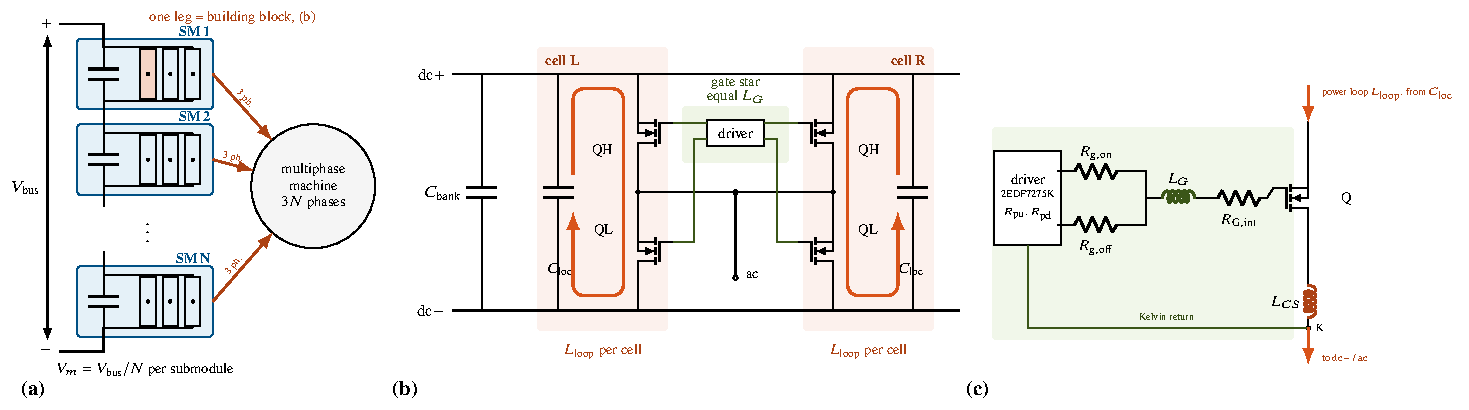
\includegraphics[width=\textwidth]{fig_spb_standalone.pdf}
\caption{(a) SPB converter, (b) building block with the centre driver and two mirrored cells, (c) gate and power circuit of one transistor with the Kelvin connection K, which limits the common-source inductance $L_{CS}$ to the package and pad.}
\label{fig:circuit}
\end{figure}

\section{Layout: current distribution and switching loss}
Paralleled GaN transistors share the conduction current well because $R_\mathrm{DS(on)}$ has a positive temperature coefficient; the static current at the end of a pulse is 59--60\,A per transistor in every case of Fig.~\ref{fig:sharing}. The switching transients, however, are set by the gate circuit of each transistor, and any asymmetry moves switching energy into one device (Fig.~\ref{fig:sharing}, Table~\ref{tab:sharing}).

\begin{figure}[H]
\centering
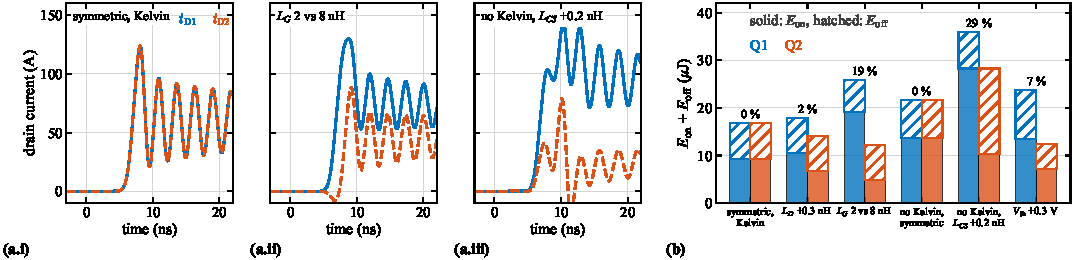
\includegraphics[width=\textwidth]{fig_sharing.pdf}
\caption{Two paralleled EPC2361 (LTspice, 75\,V, 120\,A): (a) drain currents at turn-on for the symmetric layout, a gate-loop mismatch and a common-source mismatch without Kelvin; (b) turn-on (solid) and turn-off (hatched) energy of both transistors for one asymmetry at a time, with the dynamic imbalance.}
\label{fig:sharing}
\end{figure}

\begin{table}[H]
\centering\small
\caption{Sensitivity of sharing and switching energy to one asymmetry at a time}
\label{tab:sharing}
\begin{tabular}{@{}lccccl@{}}
\toprule
Case & $I_\mathrm{diff}$ & $E_\mathrm{on}$ Q1/Q2 & $E_\mathrm{off}$ Q1/Q2 & mechanism \\
 & [\%] & [\textmu J] & [\textmu J] & \\
\midrule
symmetric, Kelvin & 0 & 9.3 / 9.3 & 7.5 / 7.5 & -- \\
drain path +0.3\,nH & 2 & 10.5 / 6.7 & 7.4 / 7.5 & slower $di/dt$ in one branch \\
gate loop 2 vs 8\,nH & 19 & 19.2 / 4.9 & 6.7 / 7.4 & one gate delayed by $\approx\Delta L_G/R$ \\
no Kelvin, symmetric & 0 & 13.7 / 13.7 & 8.0 / 8.0 & negative feedback, both slower \\
no Kelvin, $L_{CS}$ +0.2\,nH & 29 & 28.3 / 10.2 & 7.7 / 18.0 & feedback stronger in one device \\
$V_\mathrm{th}$ +0.3\,V & 7 & 13.6 / 7.1 & 10.2 / 5.3 & device spread, not layout \\
\bottomrule
\end{tabular}
\end{table}

Three layout rules follow, in order of importance:
\begin{enumerate}\itemsep1pt
\item \textbf{Kelvin source for every transistor.} A common-source inductance acts as negative feedback on the gate; it slows the switching when it is equal, and it unbalances it when it is not. The Q3D extraction of the combined power and gate model gives \LcsKel\,nH with a Kelvin via in each source pad and \LcsNoK\,nH when the driver ground is taken from the dc$-$ plane; even \LcsKel\,nH induces about 0.8\,V at 27\,A/ns, but equally in both transistors.
\item \textbf{Equal gate loops.} A mismatch $\Delta L_G$ delays one gate by roughly $\Delta L_G/R_G$, comparable to the 4\,ns current rise. A side-mounted driver would give 2.0 and 7.7\,nH to the near and far transistor (Q3D), i.e., close to the 2 versus 8\,nH case; the centre driver gives \LgateCs\,nH to both.
\item \textbf{Power-loop symmetry} matters less: 0.3\,nH in one drain path gives 2\,\% imbalance, mainly a shift of $E_\mathrm{on}$. Threshold spread (7\,\%) is a device property and can only be reduced by selection.
\end{enumerate}

\section{Driver output stage: sink and source}
\begin{figure}[H]
\centering
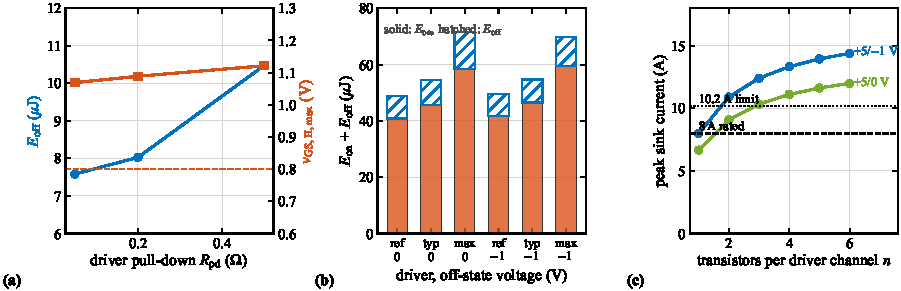
\includegraphics[width=\textwidth]{drv_output_stage.pdf}
\caption{(a) Turn-off energy and high-side gate bump against the driver pull-down resistance (0\,V off-state). (b) Switching energy for the LT8418-like reference (0.6/0.2\,$\Omega$), the 2EDF7275K with typical (0.85/0.35\,$\Omega$) and maximum (1.6/0.75\,$\Omega$) output resistance, at 0 and $-1$\,V off-state. (c) Peak sink current of one driver channel against the number of transistors it drives (0.35\,$\Omega$ pull-down, 0.4\,$\Omega$ internal gate resistance, no external turn-off resistor), with the 2EDF7275K rating and current limit.}
\label{fig:out}
\end{figure}
The \textbf{sink} (pull-down) path does two things: it turns the transistor off and it holds the complementary transistor off. For the turn-off, it is part of $R_\mathrm{g,off,tot}$; as long as this stays below the critical resistance $R_\mathrm{crit}=V_\mathrm{pl}Q_\mathrm{oss,tot}/(IQ_\mathrm{GD})$ (about 1.5\,$\Omega$ at 139\,A), the channel is off before $v_\mathrm{DS}$ rises and $E_\mathrm{off}$ stays small (7--8\,\textmu J); above it the turn-off becomes channel-controlled and $E_\mathrm{off}$ grows quickly (18.5, 39.6 and 78.7\,\textmu J for 2, 5 and 10\,$\Omega$ external, slow-switching study). Fig.~\ref{fig:out}a shows the same trend for the driver itself: \RpdEoffLo, \RpdEoffMid{} and \RpdEoffHi\,\textmu J for 0.05, 0.2 and 0.5\,$\Omega$. For the hold-off, in contrast, even 0.05\,$\Omega$ does not help (\RpdBumpLo\,V bump against \RpdBumpHi\,V at 0.5\,$\Omega$), because the Miller charge arrives within 4--6\,ns and the gate loop ($L_G$\,=\,1.7\,nH, $R_\mathrm{G,int}$\,=\,0.4\,$\Omega$) cannot move it in that time: $\Delta v_\mathrm{GS}\approx Q_\mathrm{GD}/C_\mathrm{GS}\approx\BmpDivider$\,V. A strong sink is therefore needed for a fast, low-loss turn-off and for holding against slower disturbances, but the fast bump has to be handled by the off-state voltage (Section~\ref{sec:neg}).

The \textbf{source} (pull-up) sets, together with $R_\mathrm{g,on}$, the turn-on speed and $E_\mathrm{on}$. The 2EDF7275K has a weaker pull-up than the reference (0.85 against 0.6\,$\Omega$), which raises $E_\mathrm{on}$ by about 11\,\% (typical) and 43\,\% (maximum resistance, Fig.~\ref{fig:out}b); $R_\mathrm{g,on}$ can be reduced from 2 to 1.5\,$\Omega$ to compensate, as long as the high-side overshoot stays below 90\,V.

The \textbf{peak sink current} is often the binding rating. With $-1$\,V and no external turn-off resistor, one channel driving two transistors must sink about $6\,\mathrm{V}/(0.35+0.4/2)\,\Omega\approx\SnkTwo$\,A (Fig.~\ref{fig:out}c), more than the 8\,A rating of the 2EDF7275K; its active current limit (about 10\,A) then shapes the turn-off. An external turn-off resistor of about 0.4\,$\Omega$ per transistor limits the peak to 8\,A at the cost of a slightly slower turn-off (per-transistor $R_\mathrm{g,off,tot}\approx1.5\,\Omega\approx R_\mathrm{crit}$ at the peak current); this has to be confirmed with a current-limited driver model.

\section{Negative off-voltage}\label{sec:neg}
\begin{figure}[H]
\centering
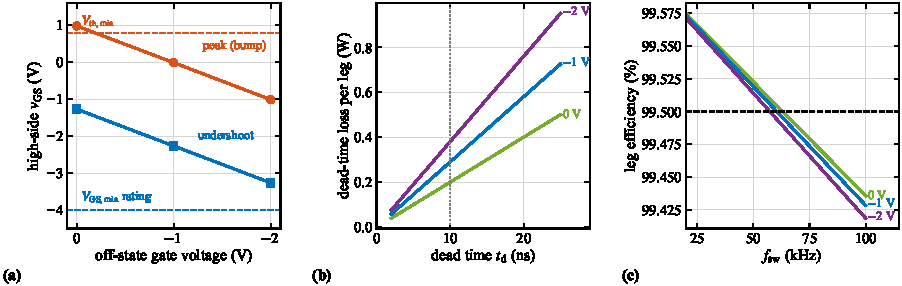
\includegraphics[width=\textwidth]{drv_negative_rail.pdf}
\caption{(a) Peak (bump) and minimum (undershoot) high-side gate voltage against the off-state voltage (75\,V, 141\,A). (b) Dead-time loss per leg against dead time for 0, $-1$ and $-2$\,V (50\,kHz, 100\,A$_\mathrm{rms}$). (c) Leg efficiency against switching frequency with the 2EDF7275K (typical) for the three off-state voltages, including the change of the switching energies and the dead-time loss.}
\label{fig:neg}
\end{figure}
A negative off-state voltage shifts the whole high-side gate waveform down by the same amount (Fig.~\ref{fig:neg}a): the peak falls from 0.99 to \BmpNegOneSF\,V at $-1$\,V and to \BmpNegTwoSF\,V at $-2$\,V, while the bump amplitude itself stays about 1\,V. The price appears in three places:
\begin{itemize}\itemsep1pt
\item \textbf{Dead-time loss.} A GaN HEMT conducts in reverse through its channel with $v_\mathrm{SD}\approx V_\mathrm{th}+|v_\mathrm{GS,off}|+iR$; every volt of negative bias adds one volt to the reverse drop during the dead time. At 10\,ns and 50\,kHz the dead-time loss per leg rises from \DeadZero{} to \DeadOne{} and \DeadTwo\,W (Fig.~\ref{fig:neg}b); it grows linearly with the dead time (\DeadOneFive{} and \DeadOneTwenty\,W at 5 and 20\,ns with $-1$\,V) and with $f_\mathrm{sw}$, so a negative bias should be combined with a short, well-controlled dead time.
\item \textbf{Undershoot.} When the complementary transistor turns off, the gate is pulled further negative by the Miller current: $-1.3$, $-2.3$ and $-3.3$\,V for 0, $-1$ and $-2$\,V, against an absolute maximum of $-4$\,V; $-2$\,V leaves only 0.7\,V.
\item \textbf{Switching energies.} The faster turn-off slightly raises the low-side overshoot (86.5 $\rightarrow$ 88.7\,V at $-1$\,V) and the larger gate swing (6\,V) increases the gate charge; the switching energy changes by less than 2\,\%.
\end{itemize}
The net effect on the leg efficiency is about 0.01\,\% per volt at 50\,kHz (Fig.~\ref{fig:neg}c). $-1$\,V gives 0.8\,V margin to $V_\mathrm{th,min}$ and is selected. The bias requires a driver whose output ground can be referenced below the transistor source, i.e., an isolated output with a split supply (2EDF7275K: +5\,V/$-$1\,V from a 6\,V isolated rail and a Zener around the Kelvin source); 5\,V-class bootstrap half-bridge drivers (maximum supply about 5.9\,V) cannot provide it without losing on-state gate voltage.

\section{More transistors in parallel: why more drivers}
\begin{figure}[H]
\centering
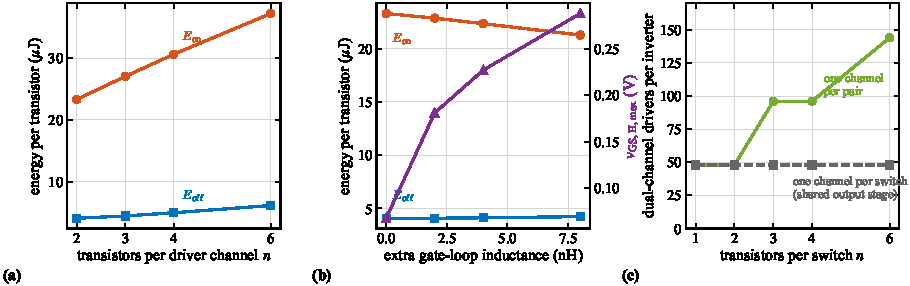
\includegraphics[width=\textwidth]{drv_scaling.pdf}
\caption{(a) Switching energy per transistor when one driver channel is shared by $n$ transistors (2EDF7275K typical, $-1$\,V, same current per transistor; the output resistance per transistor scales with $n$). (b) Effect of a longer gate loop (extra inductance in every branch, e.g., a one-driver tree for more devices): switching energy and high-side gate peak. (c) Number of dual-channel drivers of the 48-leg inverter for one channel per pair of transistors and for one channel per switch.}
\label{fig:scale}
\end{figure}
Driving more paralleled transistors from one driver channel fails for four reasons:
\begin{enumerate}\itemsep1pt
\item \textbf{Symmetry.} A driver on a mirror line reaches exactly two transistors through identical branches. A third branch cannot be made identical in a planar layout whose gate loops also have to stay orthogonal to the power loops, and any mismatch moves switching energy into one device (Table~\ref{tab:sharing}).
\item \textbf{Output resistance.} The output stage is shared, so the effective pull-up and pull-down resistance per transistor grows with $n$. At the same current per transistor, $E_\mathrm{on}$ rises from \ShEonTwo{} to \ShEonThree, \ShEonFour{} and \ShEonSix\,\textmu J and $E_\mathrm{off}$ from \ShEoffTwo{} to \ShEoffSix\,\textmu J per transistor for $n$\,=\,2, 3, 4, 6 (Fig.~\ref{fig:scale}a): the advantage of paralleling is partly lost in switching loss.
\item \textbf{Peak current.} The peak sink current grows to \SnkFour\,A for four transistors at $-1$\,V (Fig.~\ref{fig:out}c), far above the 8\,A rating; limiting it with resistors slows the turn-off further.
\item \textbf{Gate-loop length.} A tree that reaches four transistors from one driver is longer. An extra 2, 4 and 8\,nH per branch raises the high-side peak from \LgBumpZero{} to \LgBumpTwo, \LgBumpFour{} and \LgBumpEight\,V, eating into the margin of the negative bias, and reduces the turn-on $dv/dt$ (16.6 to 12.9\,V/ns); it also increases the gate ringing and the risk of exceeding the +6\,V gate rating at turn-on, which was not evaluated here.
\end{enumerate}
The building block therefore scales in pairs: one driver channel per pair of transistors in a star, three transistors per switch need a second channel, and four are built as two two-transistor structures with two drivers (Fig.~\ref{fig:scale}c). Going from two to three or four transistors per switch doubles the drivers of the inverter from 48 to 96, together with their isolated supplies; with the leg loss falling by only 1.3--1.7\,W from two to three or four transistors (design paper), two transistors per switch remain the best choice.

\section{Driver comparison}
\begin{table}[H]
\centering\small
\caption{Gate drivers considered (values from the datasheets in \texttt{Datasheet/} where available; n/a: not checked)}
\label{tab:drivers}
\setlength{\tabcolsep}{3.5pt}
\begin{tabularx}{\textwidth}{@{}lXXXX@{}}
\toprule
 & LT8418 (model) & 2EDL5013U2D & uP1966E (EPC90156) & \textbf{2EDF7275K} \\
\midrule
Type & 100\,V half bridge, bootstrap & 120\,V half bridge, bootstrap & 80\,V half bridge, bootstrap & dual-channel isolated (1.5\,kV functional) \\
Pull-up / pull-down & 0.6 / 0.2\,$\Omega$ (model value) & HS 0.9 / 0.5\,$\Omega$, LS 1.5 / 0.5\,$\Omega$ & n/a & 0.85 / 0.35\,$\Omega$ typ., 1.6 / 0.75\,$\Omega$ max \\
Peak source / sink & n/a & 2--3\,A / 5\,A & n/a & 4\,A / 8\,A \\
Miller clamp & n/a & yes, 0.5\,V, 5\,ns delay, 7\,A & n/a & no \\
Supply & n/a & 4.5--5.5\,V (5.9\,V abs.\ max) & 5\,V gate drive & 4.5--20\,V, UVLO 4\,V \\
Negative off-voltage & no & no (supply limit) & no & yes, split isolated supply \\
Use in this work & reference model & bootstrap alternative without bias & EPC reference board (1\,$\Omega$/0.47\,$\Omega$) & selected \\
\bottomrule
\end{tabularx}
\end{table}

\section{Recommendations}
\begin{enumerate}\itemsep1pt
\item Keep the centre-driver star with Kelvin vias in every source pad; route the Kelvin return directly under the gate trace (\LgateCs\,nH, \LcsKel\,nH).
\item Use the 2EDF7275K, one channel per switch star, with a +5/$-$1\,V split isolated supply; keep the dead time short (5--10\,ns) to limit the dead-time loss.
\item Limit the peak sink current to the 8\,A rating (about 0.4\,$\Omega$ external turn-off resistor per transistor) or confirm the driver current limit with a current-limited model.
\item Scale paralleling in pairs, one driver channel per pair; do not drive more than two transistors from one channel.
\item On the prototype, measure the high-side gate with an isolated probe at the gate pad, and keep footprints for a gate--source capacitor as a fallback.
\end{enumerate}

\noindent\small Files: \texttt{simulation/bb\_spice/BB\_bump.inc} with \texttt{BB\_bump.cir}, \texttt{BB\_bump\_rpd.cir}, \texttt{BB\_2EDF7275K.cir}, \texttt{BB\_drv\_share.cir}, \texttt{BB\_gate\_len.cir}; \texttt{simulation/sharing/paper\_run}; \texttt{simulation/bb\_q3d/bb\_q3d\_cs.py}; \texttt{scripts/gate\_driver\_report.py}.
\end{document}
